\begin{prob}
	Consider the following directed graph.
        \begin{center}
                    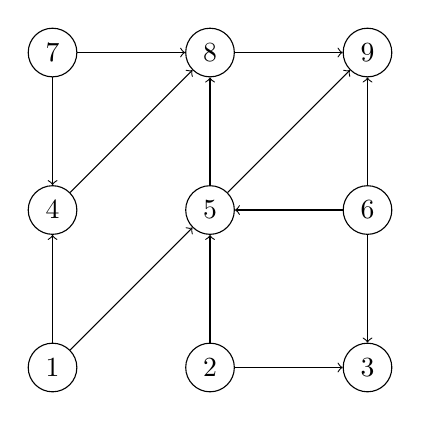
\begin{tikzpicture}
                        \foreach \i in {1,...,9}{
                            \pgfmathparse{mod(\i-1,3)} \pgfmathresult %displays 2.0
                            \pgfmathtruncatemacro{\x}{\pgfmathresult}

                            \pgfmathtruncatemacro{\y}{(\i-1)/3}

                            \node[draw, circle] (n\i) at (2*\x, 2*\y) {$\i$};
                        }

                        \foreach \u/\v in {%
                            2/3,
                            2/5,
                            6/5,
                            1/4,
                            5/9,
                            5/8,
                            8/9,
                            6/9,
                            4/8,
                            7/4,
                            7/8,
                            6/3,
                            1/5%
                            }{
                            \draw (n\u) edge[->] (n\v);
                        }

                    \end{tikzpicture}
                \end{center}
	\begin{subprobset}
	    \begin{subprob}
		Run Full\textunderscore DFS on the graph above. Make a bold arrow from node $u$ to node $v$ if $u$ is
                the predecessor of node $v$ in DFS. Use the convention
                that nodes are processed in ascending order by
                label.
		\begin{soln}
		    \begin{center}
                    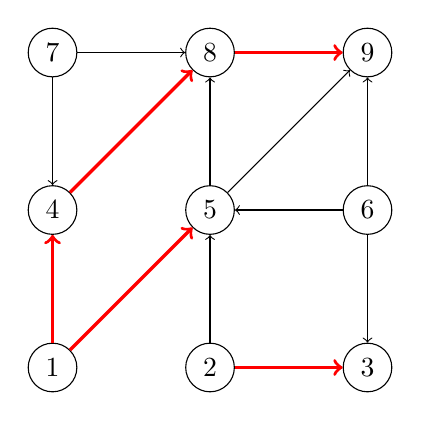
\begin{tikzpicture}
                        \foreach \i in {1,...,9}{
                            \pgfmathparse{mod(\i-1,3)} \pgfmathresult %displays 2.0
                            \pgfmathtruncatemacro{\x}{\pgfmathresult}

                            \pgfmathtruncatemacro{\y}{(\i-1)/3}

                            \node[draw, circle] (n\i) at (2*\x, 2*\y) {$\i$};
                        }

                        \foreach \u/\v in {%
                            6/3,
                            2/5,
                            6/5,
                            5/9,
                            5/8,
                            6/9,
                            7/4,
                            7/8%
                            }{
                            \draw (n\u) edge[->] (n\v);
                        }

			\foreach \u/\v in {%
                            1/4,
                            8/9,
                            4/8,
                            2/3,
                            1/5%
                            }{
                            \draw (n\u) edge[very thick, red,->] (n\v);
                        }

                    \end{tikzpicture}
                \end{center}
		\end{soln}
	    \end{subprob}
  	    \begin{subprob}
		Fill in the table below so that it contains the start and
                finish times of each node after a Full\textunderscore DFS is performed on the above graph. Assume node 1 as the source for the first DFS call.
                Begin your start times with 1.
		\begin{center}
                    \begin{minipage}{0.4\textwidth}
                    \centering
                    \begin{tabular}{ccc}
                        Node & Start & Finish\\
                        1 & \inlineresponsebox[.5in]{1} & \inlineresponsebox[.5in]{10} \\
                        2 & \inlineresponsebox[.5in]{11} & \inlineresponsebox[.5in]{14} \\
                        3 & \inlineresponsebox[.5in]{12} & \inlineresponsebox[.5in]{13} \\
                        4 & \inlineresponsebox[.5in]{2} & \inlineresponsebox[.5in]{7} \\
                        5 & \inlineresponsebox[.5in]{8} & \inlineresponsebox[.5in]{9} \\
                    \end{tabular}
                    \end{minipage}%
                    \begin{minipage}{0.4\textwidth}
                    \centering
                    \begin{tabular}{ccc}
                        Node & Start & Finish\\
                        6 & \inlineresponsebox[.5in]{15} & \inlineresponsebox[.5in]{16} \\
                        7 & \inlineresponsebox[.5in]{17} & \inlineresponsebox[.5in]{18} \\
                        8 & \inlineresponsebox[.5in]{3} & \inlineresponsebox[.5in]{6} \\
                        9 & \inlineresponsebox[.5in]{4} & \inlineresponsebox[.5in]{5} \\
                    \end{tabular}
                    \end{minipage}
                \end{center}
	    \end{subprob}
  	    % \begin{subprob}
		% Topologically sort the vertices of the graph.
		% \begin{responsebox}{2in}
		%     2,6,3,7,1,5,4,8,9
		% \end{responsebox}
	    % \end{subprob}
	\end{subprobset}

    \end{prob}
